\documentclass[aspectratio=169]{beamer}
\setbeamertemplate{navigation symbols}{}
\usepackage{color,amsmath,comment, subfigure}
\usepackage{booktabs}
\usepackage{url}

%\setbeameroption{show notes}

%%%%%%%%%%%%%%%%%%%%%%%%%%
\title[]{Class 14: Strength of weak ties}
\author[]{Matthew J. Salganik}
\institute[]{Sociology 204: Social Networks\\Princeton University}
\date[]{
1/2 Strength of weak ties for individuals and groups
\vfill

\begin{flushleft}
\vspace{0.6in}

\includegraphics[width=0.1\textwidth]{figures/cc.png}
\end{flushleft}
}

\begin{document}
%%%%%%%%%%%%%%%%%%%%%%%%%%%
\frame{\titlepage}
%%%%%%%%%%%%%%%%%%%%%%%%%%%
\begin{frame}

\begin{center}
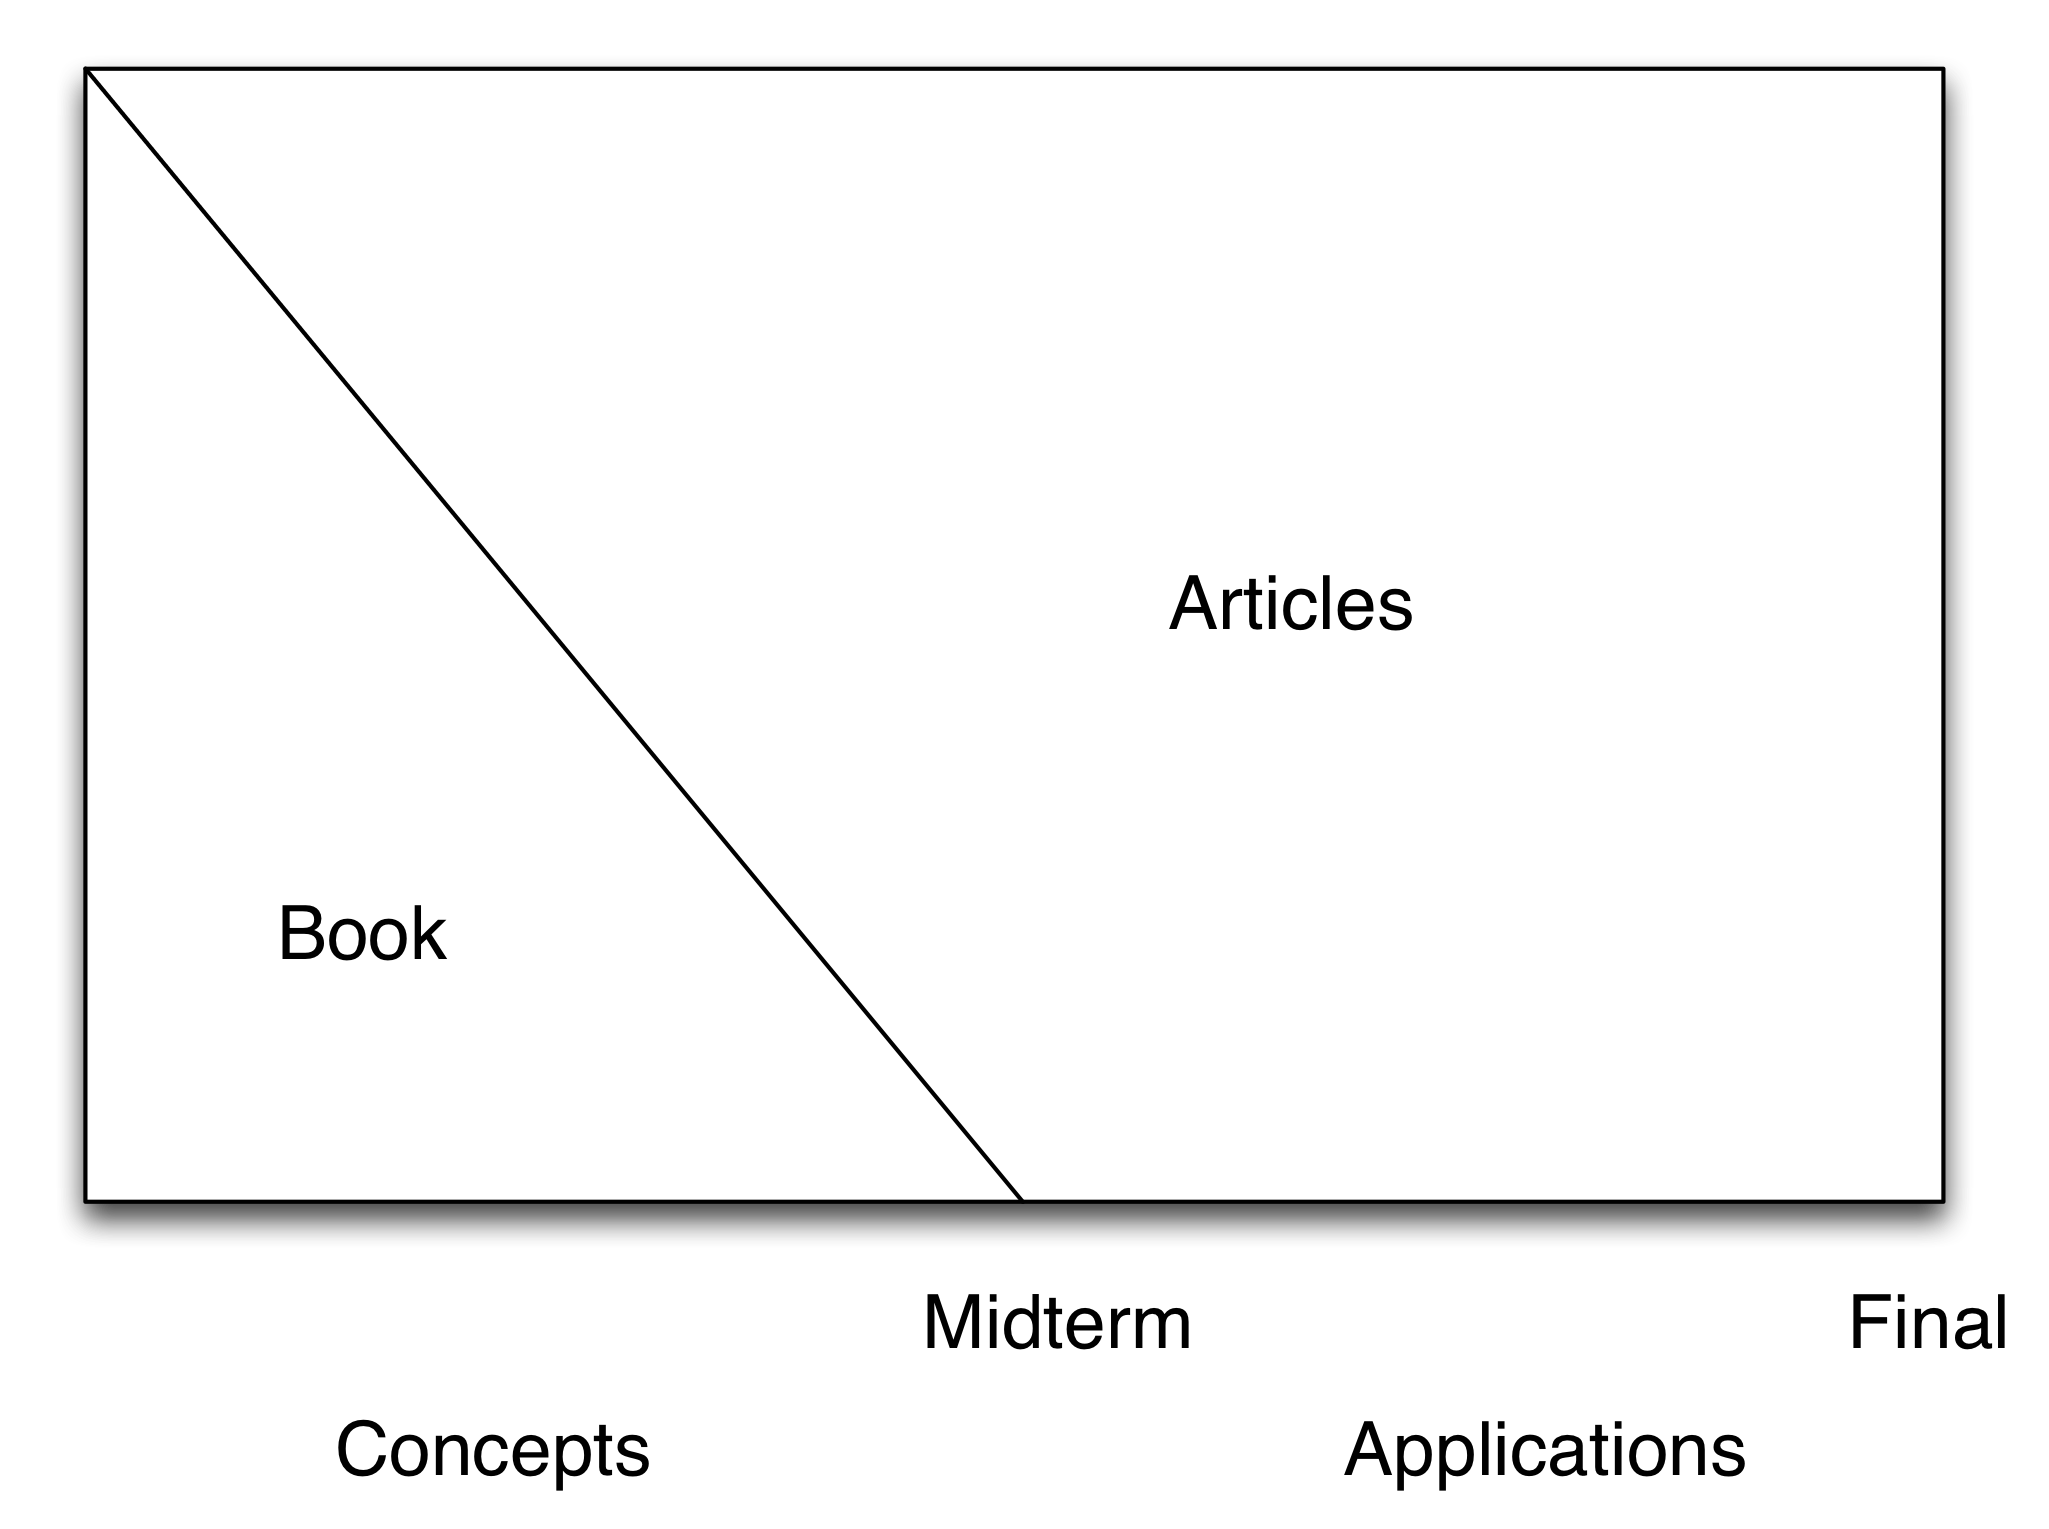
\includegraphics[width=0.75\textwidth]{figures/class_structure}
\end{center}

\end{frame}
%%%%%%%%%%%%%%%%%%%%%%%%%
\begin{frame}

\begin{itemize}
\item Students will be able to \textit{describe} the major ideas and models used in the study of networks.
\item Students will be able to \textit{describe} the interconnections between the major ideas and models used in the study of networks.
\item Students will be able to \textit{use} the major ideas and models used in the study of networks to gain insight into real-world phenomena.
\item Students will be able to \textit{evaluate} real, modern research that connects the major ideas and models of networks to real-world phenomena.
\end{itemize}

\end{frame}
%%%%%%%%%%%%%%%%%%%%%%%%%%%
\begin{frame}

Strength of weak ties is a classic. \pause

\begin{center}
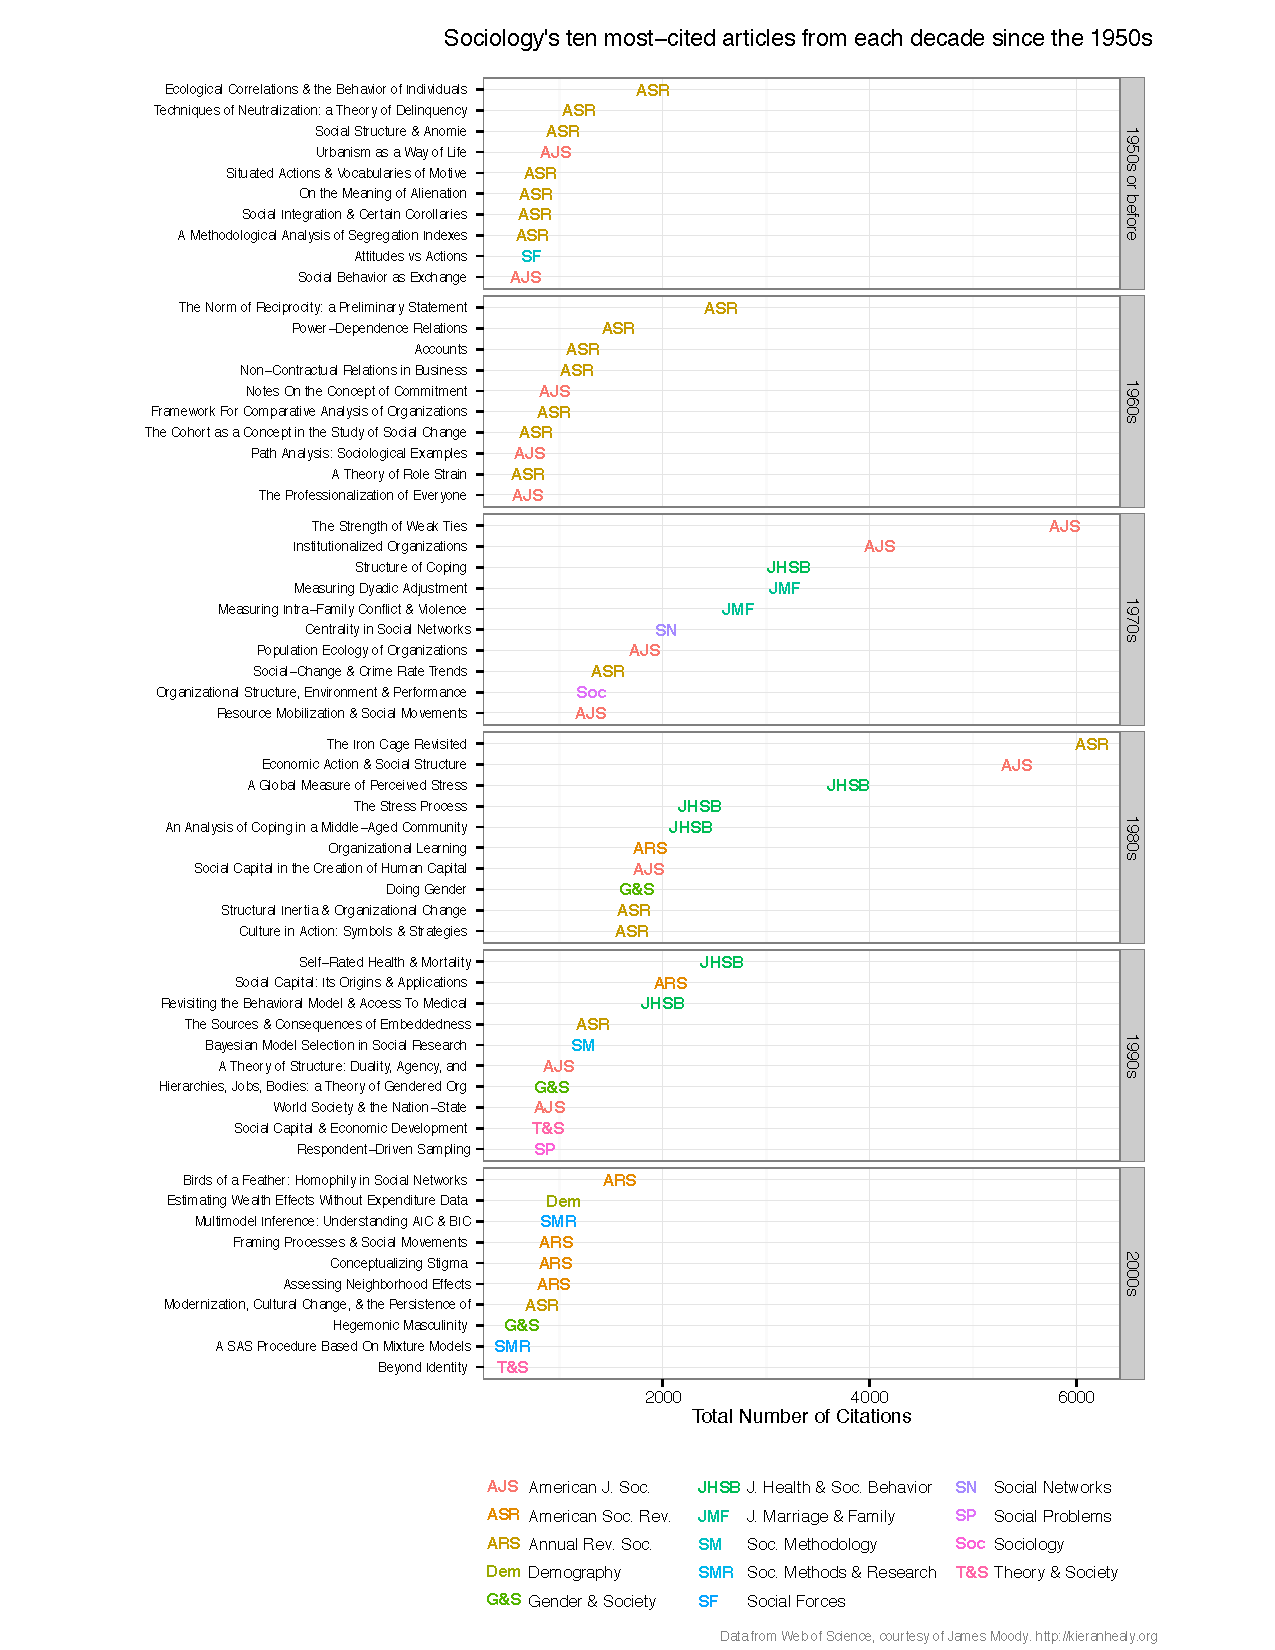
\includegraphics[height=0.85\textheight]{figures/cite-dotplot-by-decade-grouped-prod}
\end{center}

\vfill
\tiny{\url{https://kieranhealy.org/blog/archives/2014/11/15/top-ten-by-decade/}}


\end{frame}
%%%%%%%%%%%%%%%%%%%%%%%%
\begin{frame}

Strength of weak ties is a classic for three reasons:
\pause
\begin{itemize}
\item one extra bit of complexity and one plausible assumption lead to surprising empirical predictions, many that turn out to be true \pause
\item connects micro rules to macro patterns (similar to Bearman et al.\ study of sexual networks) \pause
\item generates lots of new research 
\end{itemize}

\end{frame}
%%%%%%%%%%%%%%%%%%%%%%%%
\begin{frame}

\begin{center}
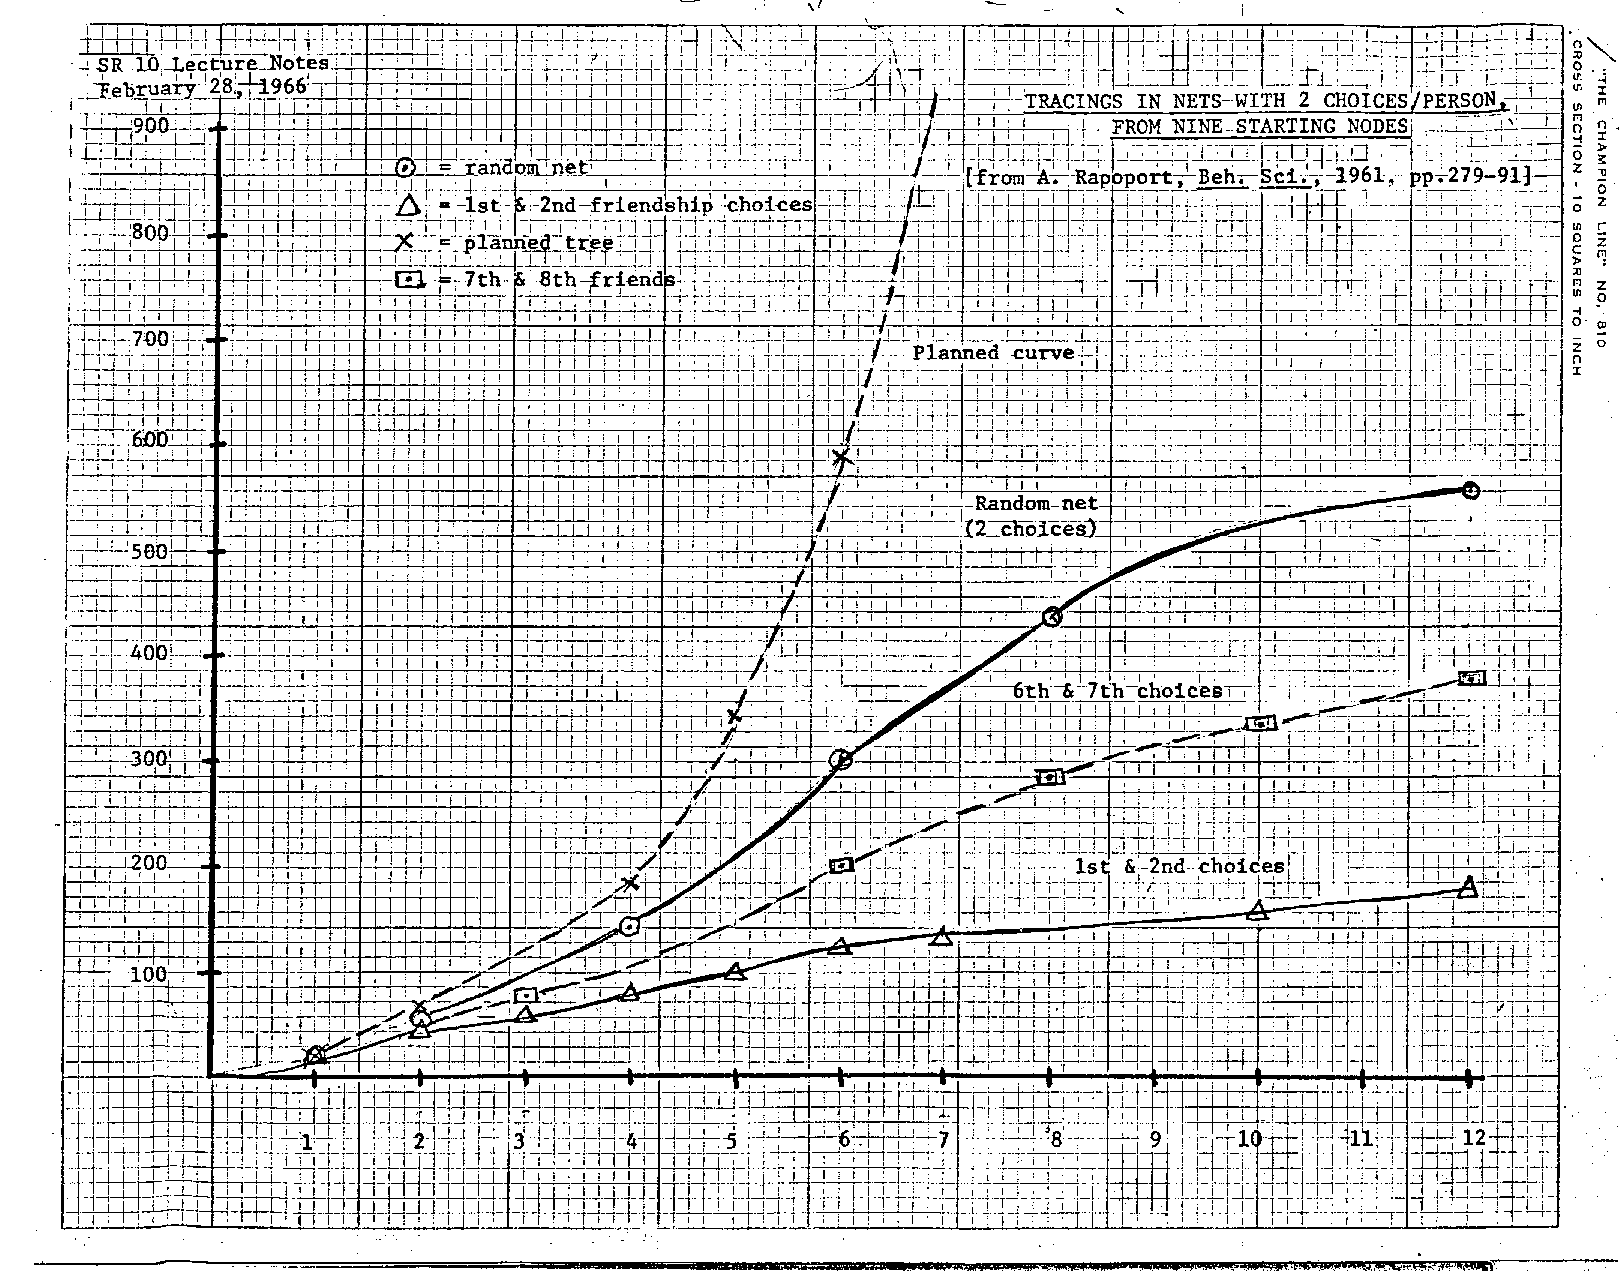
\includegraphics[width=0.6\textwidth]{figures/white_classnotes_swt}
\end{center}

\vfill
Source: From Harrison White's class in 1966
\note{ 

Choose 9 random seeds and then followed two closest friends and then those two closest friends and then their two closest friends and so on.  Repeated many times to see how many people were reached on average.\\
Then repeated but followed third and forth closest friends.\\
Then repeated but followed fifth and sixth closest friends.\\
Then repeated but followed seventh and eight closest friends.\\
RESULTS:\\
Smallest number of people were reached by first and second and largest by seventh and eighth.\\

A second historical note is that like the Watts paper, this one was also rejected by a journal initially
}

\end{frame}
%%%%%%%%%%%%%%%%%%%%%%%%%
\begin{frame}

\begin{figure}
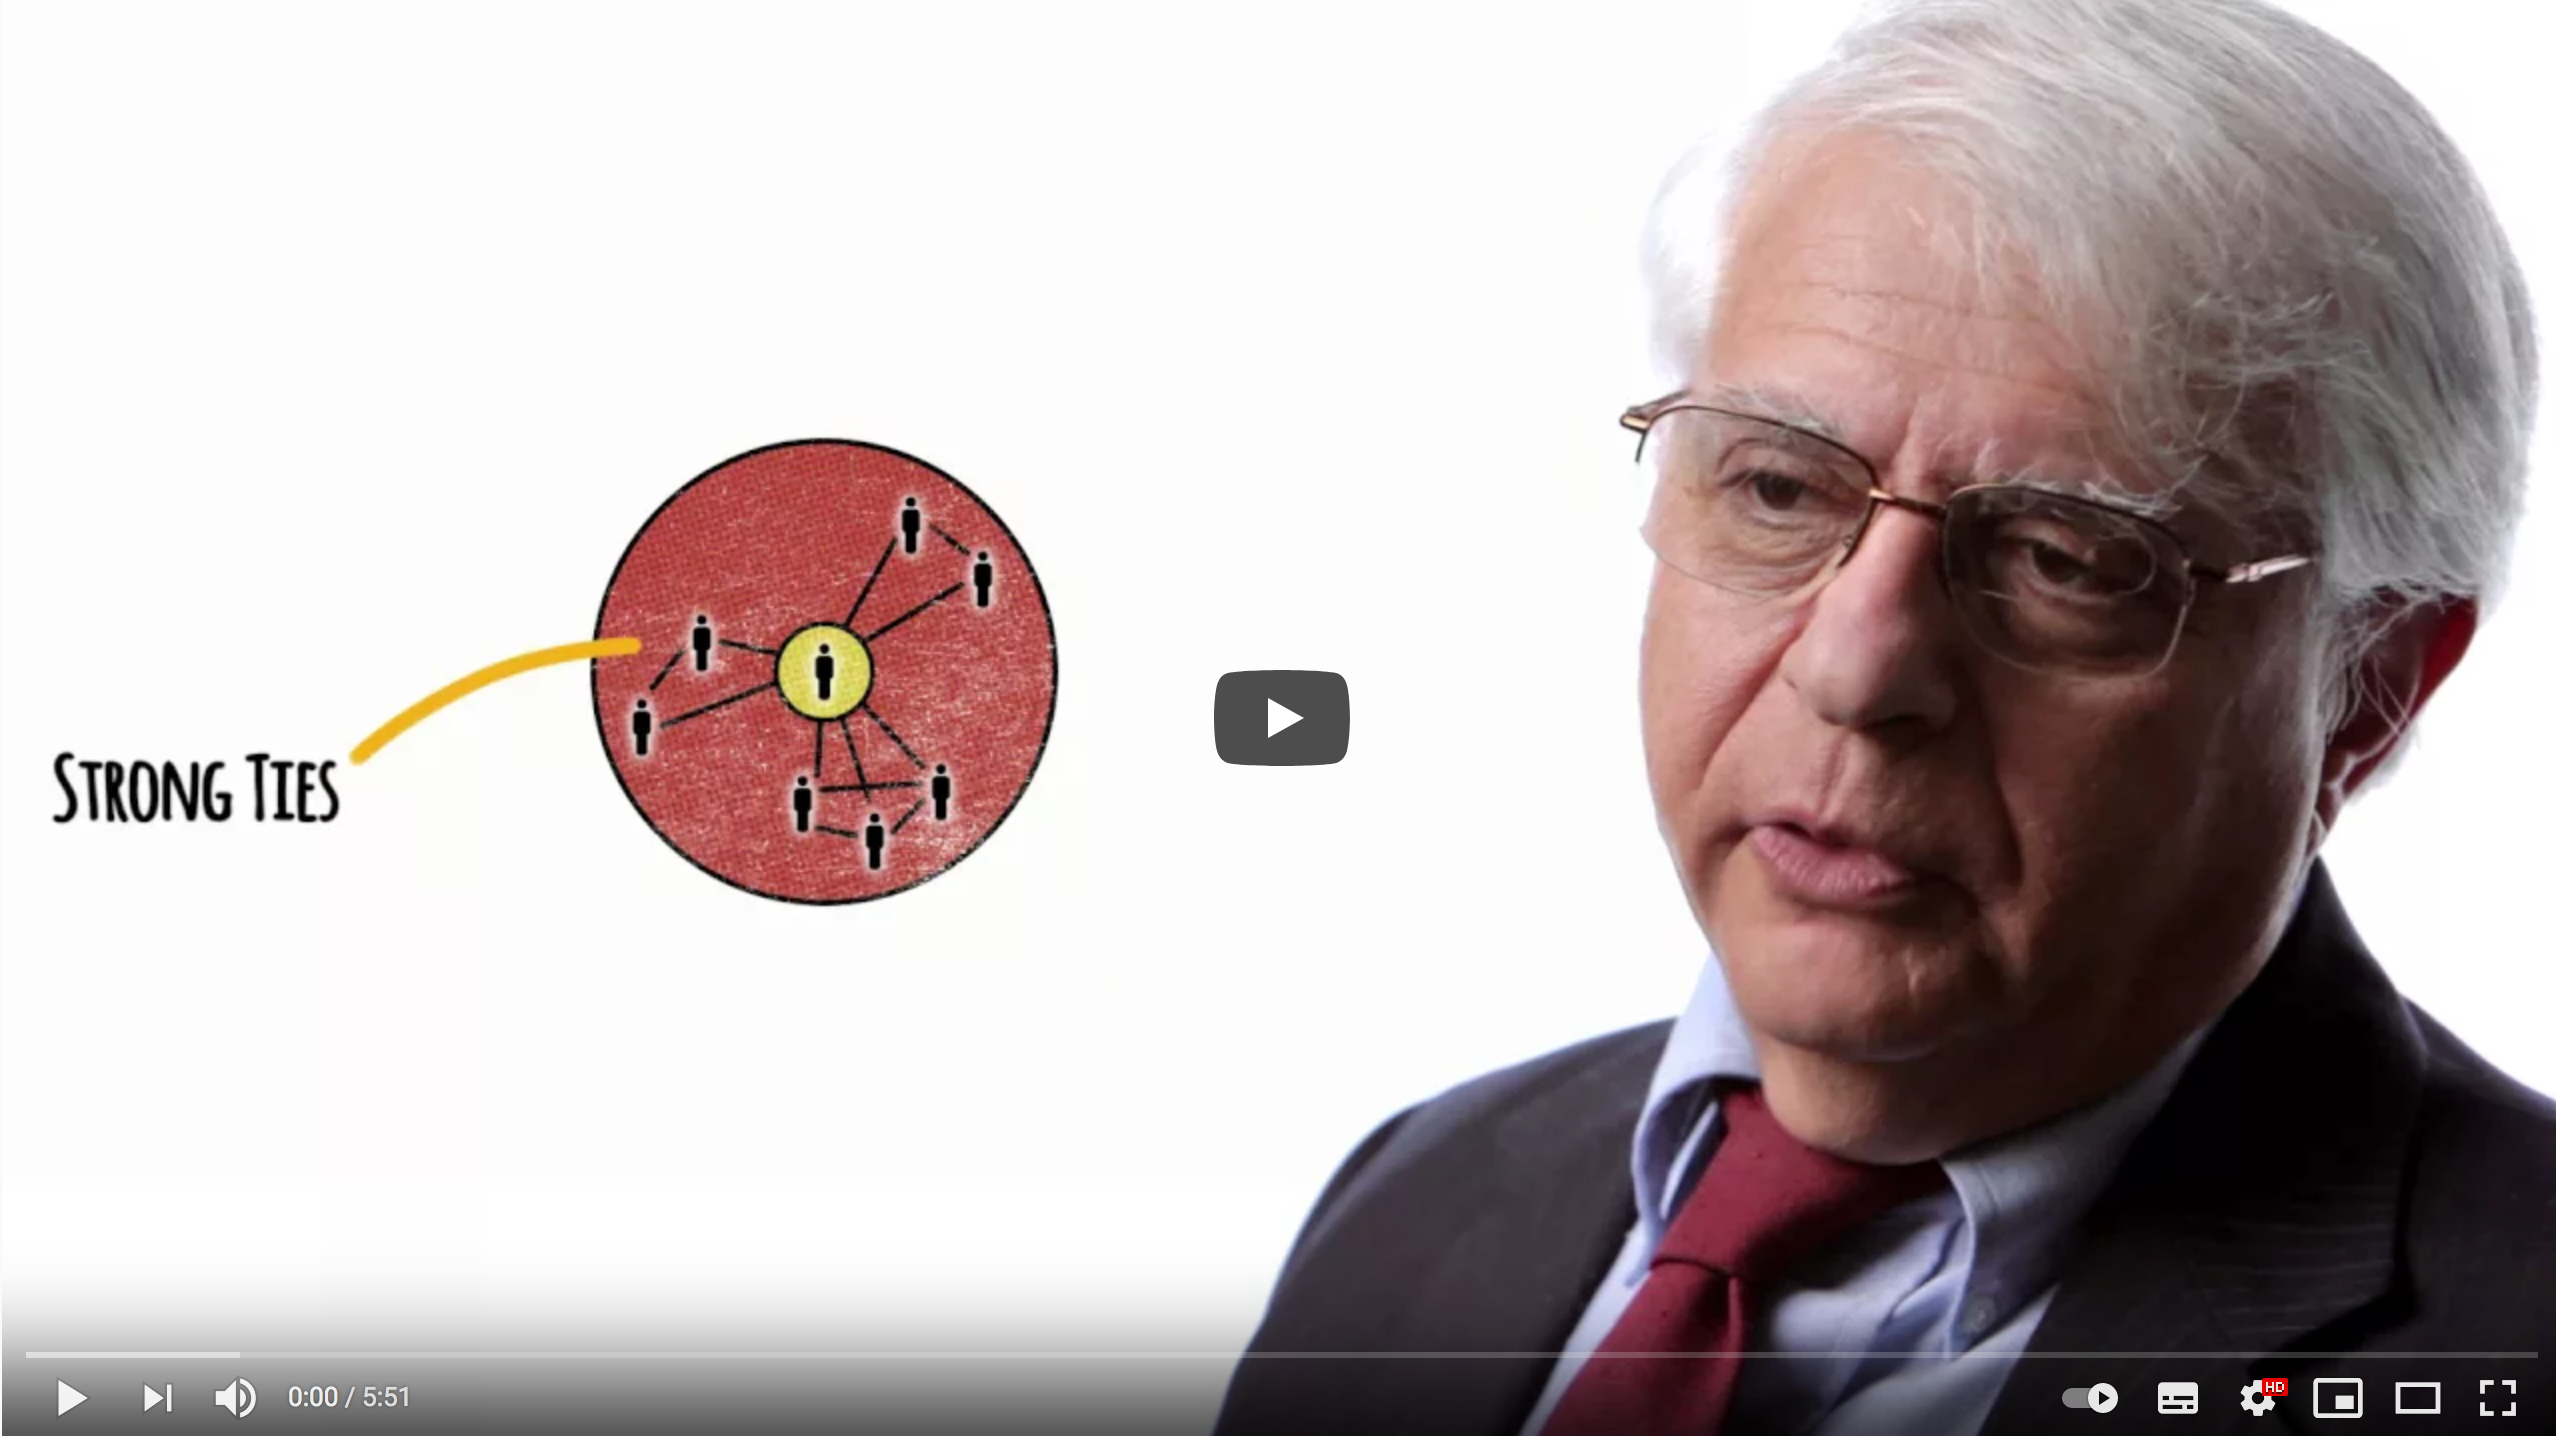
\includegraphics[width=0.6\textwidth]{figures/granovetter_swt_video}
\end{figure}

\url{https://www.youtube.com/watch?v=g3bBajcR5fE}

\end{frame}
%%%%%%%%%%%%%%%%%%%%%%%%%
\begin{frame}

``Strength of a tie is a (probably linear) combination of the amount of time, emotional intensity, the intimacy, and reciprocal services which characterize the tie.''

\end{frame}
%%%%%%%%%%%%%%%%%%%%%%%%%
\begin{frame}

Prediction:\\
The stronger the tie between two people, the more their friendship sets overlap.

\begin{figure}
  \centering
  \subfigure{
  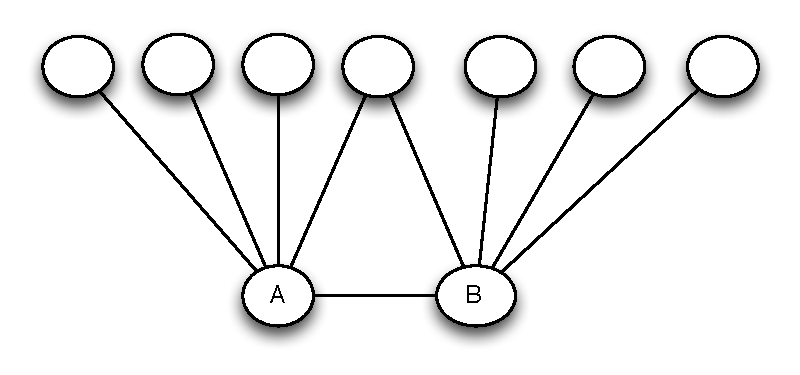
\includegraphics[width=0.4\textwidth]{figures/swt_low_overlap}}
  \hspace{0in}
  \subfigure{
  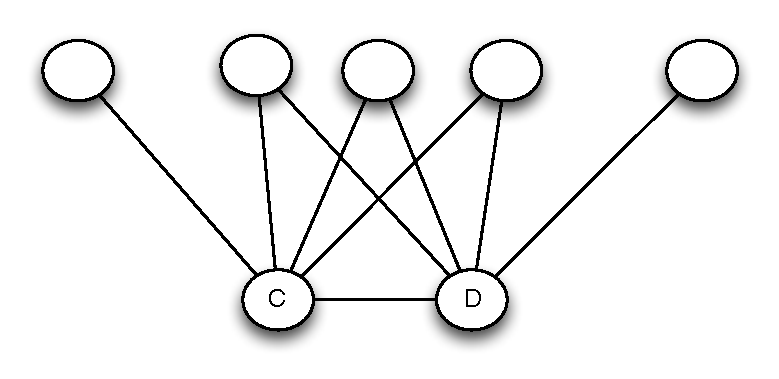
\includegraphics[width=0.4\textwidth]{figures/swt_high_overlap}}
\end{figure}

\vfill
No good data to test in 1973, but there is now (as you will see with your future homeworks).

\end{frame}
%%%%%%%%%%%%%%%%%%%%%%%
\begin{frame}

For the rest of the paper, he deals with a simplification:

\begin{itemize}
\item Old idea: tie is either present or absent
\item New idea: tie is either strong, weak, or absent
\end{itemize}

\note{

small added complexity

}

\end{frame}
%%%%%%%%%%%%%%%%%%%%%%%%
\begin{frame}

Assume no forbidden triad

\begin{figure}
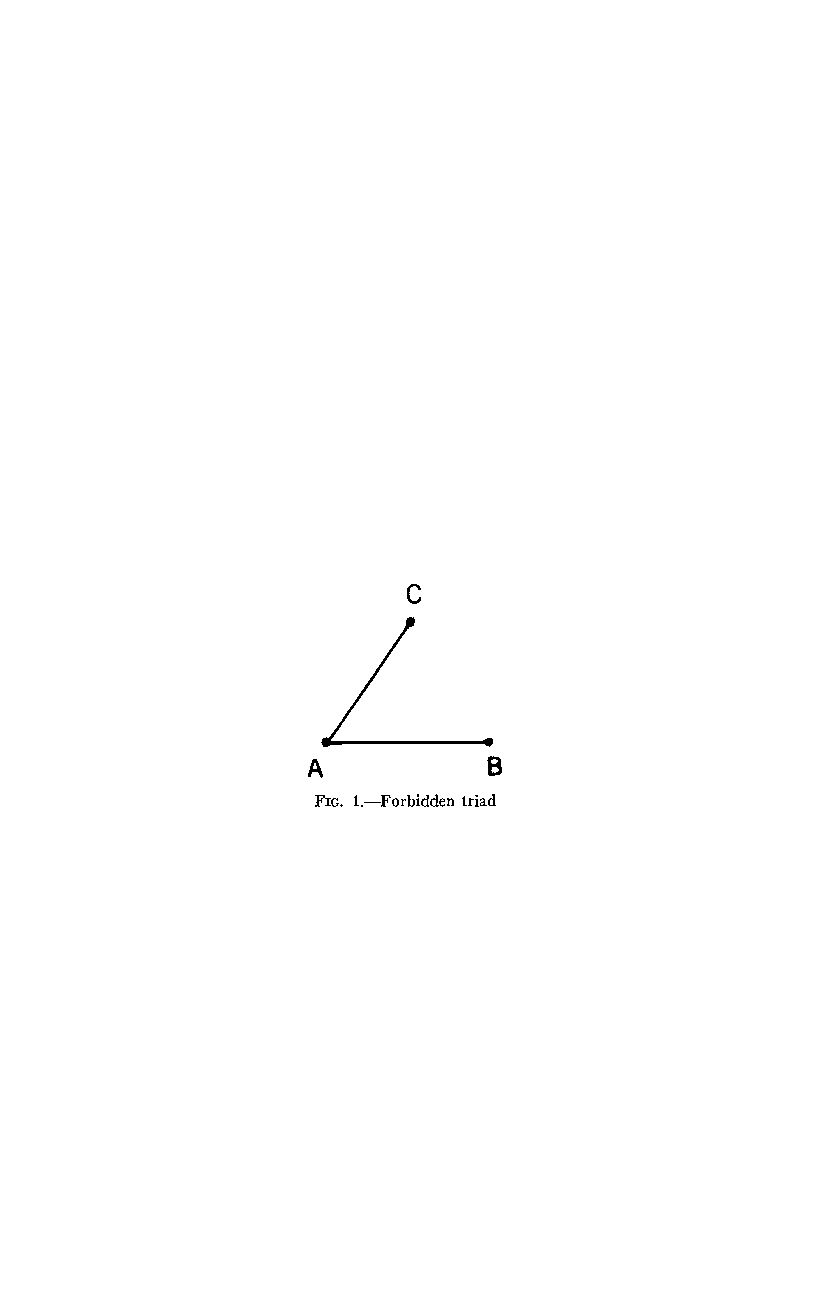
\includegraphics[width =0.5\textwidth]{figures/granovetter_strength_1973_fig1}
\end{figure}

\note{

This should remind you of clustering coefficient

}


\end{frame}
%%%%%%%%%%%%%%%%%%%%%%%%%
\begin{frame}

Except in weird cases, \emph{no strong tie is a bridge}.  Or \emph{all bridges are weak ties}.

\vfill
But, it is not the case that all weak ties are bridges.

\note{

Give an example of a weak tie that is not a bridge

}

\end{frame}
%%%%%%%%%%%%%%%%%%%%%%%%%
\begin{frame}

Bridges are probably rare, so Granovetter talks about \emph{local bridges}

\begin{figure}
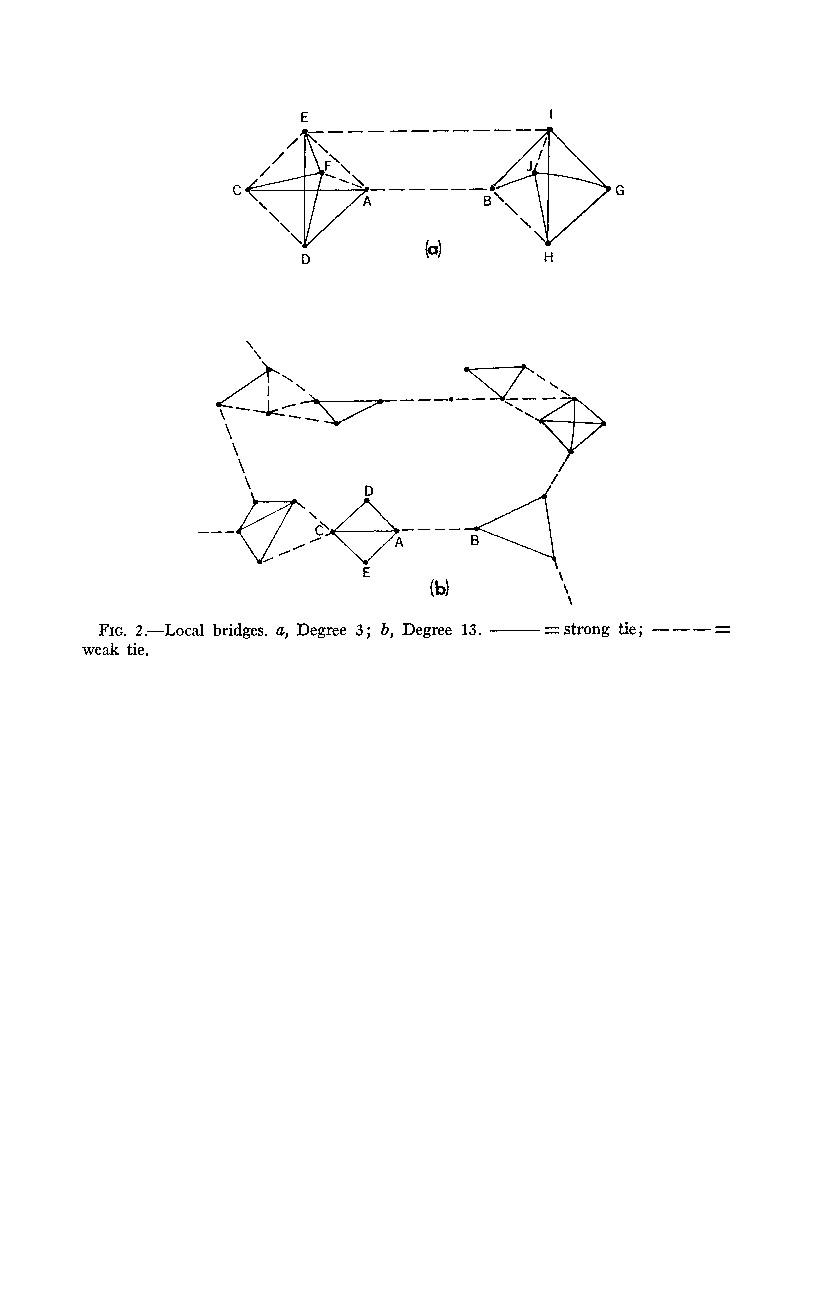
\includegraphics[width=0.5\textwidth]{figures/granovetter_strength_1973_fig2}
\end{figure}

\note{

Network bridge connects two otherwise hard to reach areas, same idea with a network bridge

}

\end{frame}
%%%%%%%%%%%%%%%%%%%%%%%%%%
\begin{frame}

``The significance of weak ties, then, would be that those which are local bridges create more and shorter paths.''

Which concept or model that we learned about does this remind you of? 

\pause

Shortcuts in beta model

\begin{figure}
\includegraphics[width=0.5\textwidth]{figures_book/3_6}
\end{figure}

\note{

With forbidden triad, shortcuts are weak

}

\end{frame}
%%%%%%%%%%%%%%%%%%%%%%%%%
\begin{frame}

Strength of weak ties for
\begin{itemize}
\item communities
\item individuals
\end{itemize}

\end{frame}
%%%%%%%%%%%%%%%%%%%%%
\begin{frame}
\frametitle{Strength of weak ties for communities}

Boston's West End was unable to resist ``urban renewal'', Granovetter argues that this is because of lack of short paths between people (think ``caveman graph'')\\

\vfill

Granovetter predicts: weak ties hold communities together and enable them to act cohesively

\note{

Talk about world where all connections are within eating clubs; rich social life, but hard to act as a campus community; lots of weak ties between groups of students make collective action possible

}

\end{frame}
%%%%%%%%%%%%%%%%%%%%%
\begin{frame}
\frametitle{Strength of weak ties for individuals}

Local bridges are most important for spreading new things.  Therefore, weak ties are important for spreading new things and receiving information.

\begin{figure}
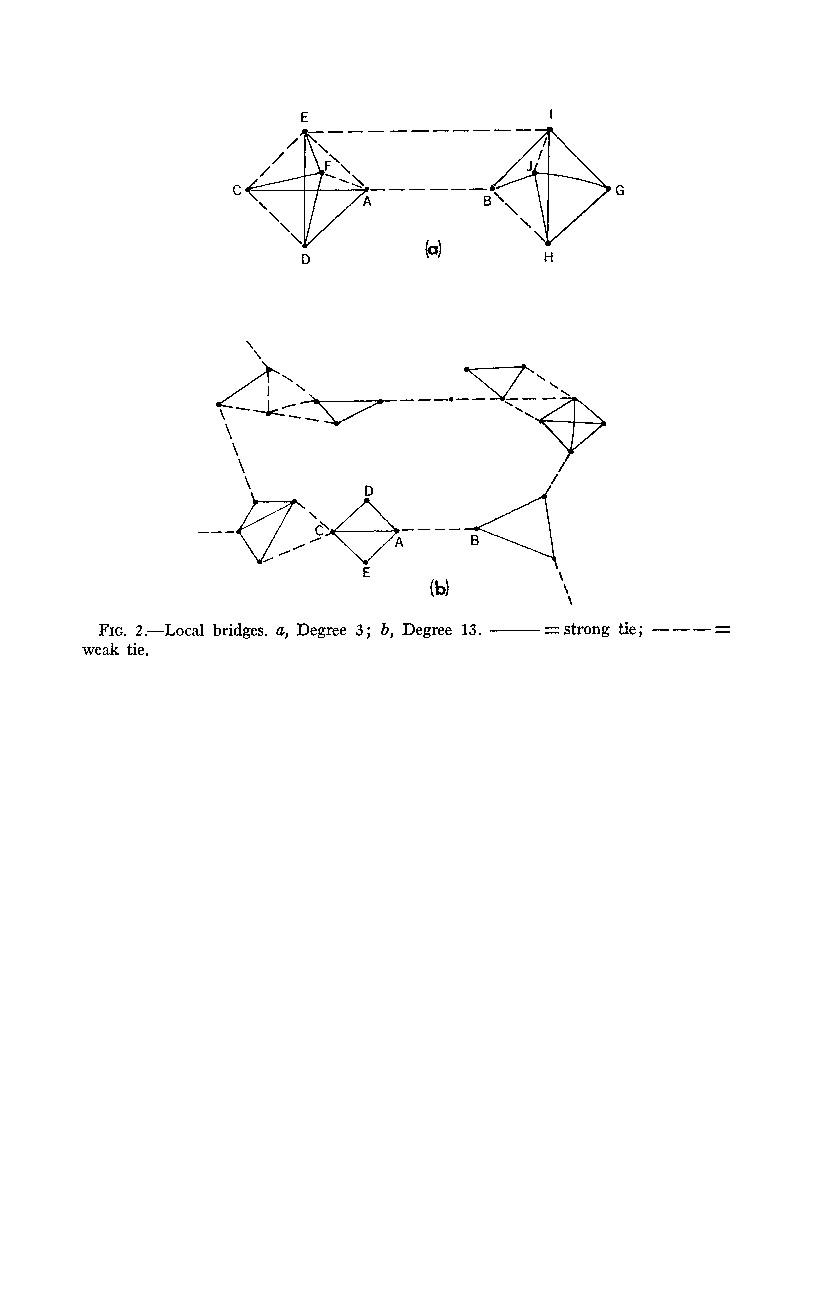
\includegraphics[width=0.5\textwidth]{figures/granovetter_strength_1973_fig2}
\end{figure}

\end{frame}
%%%%%%%%%%%%%%%%%%%%%%%%%%%
\begin{frame}

In the sample he studied (professionals in a suburb of Boston), of those who found a job through a contact, how often did they see the contact?
\begin{itemize}
\item often (at least twice a week): 17\%
\item occasionally (more than once a year but less than twice a week): 56\%
\item rarely (once a year or less): 28\%
\end{itemize}

The people you see occasionally and rarely can be the most important.

\end{frame}
%%%%%%%%%%%%%%%%%%%%%%%%%%
\begin{frame}

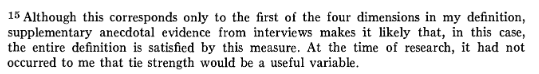
\includegraphics[width=\textwidth]{figures/granovetter_strength_1973_ft15}

\end{frame}
%%%%%%%%%%%%%%%%%%%%%%%%%%
\begin{frame}

To summarize lots of subsequent research, it is non-redundant information that is important, not weak ties.

\vfill
Therefore, a better title might have been: \emph{The strength of local bridges}

\end{frame}

\end{document}
